% The document class supplies options to control rendering of some standard
% features in the result.  The goal is for uniform style, so some attention 
% to detail is *vital* with all fields.  Each field (i.e., text inside the
% curly braces below, so the MEng text inside {MEng} for instance) should 
% take into account the following:
%
% - author name       should be formatted as "FirstName LastName"
%   (not "Initial LastName" for example),
% - supervisor name   should be formatted as "Title FirstName LastName"
%   (where Title is "Dr." or "Prof." for example),
% - degree programme  should be "BSc", "MEng", "MSci", "MSc" or "PhD",
% - dissertation title should be correctly capitalised (plus you can have
%   an optional sub-title if appropriate, or leave this field blank),
% - dissertation type should be formatted as one of the following:
%   * for the MEng degree programme either "enterprise" or "research" to
%     reflect the stream,
%   * for the MSc  degree programme "$X/Y/Z$" for a project deemed to be
%     X%, Y% and Z% of type I, II and III.
% - year              should be formatted as a 4-digit year of submission
%   (so 2014 rather than the academic year, say 2013/14 say).

\documentclass[ % the name of the author
                    author={Louis Wang},
                % the name of the supervisor
                supervisor={Dr. Qiang Liu},
                % the degree programme
                    degree={MSc},
                % the dissertation    title (which cannot be blank)
                     title={Identification of Suicide Ideation in Texts},
                % the dissertation subtitle (which can    be blank)
                  %subtitle={And those including an optional subtitle too, for good measure},
                % the dissertation     type
                      type={},
                % the year of submission
                      year={2024}]{dissertation}

\begin{document}

% =============================================================================

% This macro creates the standard UoB title page by using information drawn
% from the document class (meaning it is vital you select the correct degree 
% title and so on).


\maketitle

% After the title page (which is a special case in that it is not numbered)
% comes the front matter or preliminaries; this macro signals the start of
% such content, meaning the pages are numbered with Roman numerals.

\frontmatter

% This macro creates the standard UoB declaration; on the printed hard-copy,
% this must be physically signed by the author in the space indicated.

\makedecl

% LaTeX automatically generates a table of contents, plus associated lists 
% of figures, tables and algorithms.  The former is a compulsory part of the
% dissertation, but if you do not require the latter they can be suppressed
% by simply commenting out the associated macro.

\tableofcontents
\listoffigures
\listoftables
\listofalgorithms
\lstlistoflistings

% The following sections are part of the front matter, but are not generated
% automatically by LaTeX; the use of \chapter* means they are not numbered.

% -----------------------------------------------------------------------------

\chapter*{Abstract}


% -----------------------------------------------------------------------------

\chapter*{Supporting Technologies}

\noindent
This section lists the various technologies that I have used to implement and submit my dissertation project.

\begin{itemize}

\item Python was the main programming language used in this project. Code was developed with the version of Python 3.9. 
The following Python packages were used in the project:

\begin{itemize}
      \item {\em Scikit-Learn} for machine learning model and metrics calculation
      \item {\em Pytorch} was used as the framework of deep learning model and for building, training and testing the neural networks
      \item {\em Transformer} for its implementation of BERT and other models related to it
      \item {\em Shap} for model explanation
      \item {\em Flask} was used as the web application framework 
\end{itemize}

\item AutoDL was used for online GPU resources and remote execution of code in jupyter notebook format
 
\item \LaTeX\ was used to format the thesis, via {\em Visual Studio Code} with LaTeX Workshop. 

\item GitHub was used to store, backup and share the source code, scripts, data, etc. of this project
\url{https://github.com/Sting-Scorpion/DataScience_Project}

\end{itemize}

% -----------------------------------------------------------------------------

\chapter*{Notation and Acronyms}

\noindent
The following list of notations and acronyms will be referenced in this project:

\begin{quote}
\noindent
\begin{tabular}{lcl}
      NLP &: & Natural Language Processing \\
      XAI &: & Explainable AI \\
      SHAP &: & Shapley Additive Explanations \\
      LR &: & Logistic Regression \\
      HMM &: & Hidden Markov Methods \\
      SVM &: & Support Vector Machines \\
      KNN &: & K Nearest Neighbours \\
      CRF &: & Conditional Random Fields \\
      BoW &: & Bag-of-Words \\
      DNN &: & Deep Neural Network \\
      CNN &: & Convolutional Neural Network \\
      RNN &: & Recurrent Neural Networks \\
      LSTM &: & Long Short-Term Memory \\
      BiLSTM &: & Bidirectional Long Short-Term Memory \\
      BERT &: & Bidirectional Encoder Representations from Transformers \\
      GPU &: & Graphics Processing Unit \\
      ${\mathcal H}( x )$ &: & the Hamming weight of $x$ \\
\end{tabular}
\end{quote}

% -----------------------------------------------------------------------------

\chapter*{Acknowledgements}

\noindent

% =============================================================================

% After the front matter comes a number of chapters; under each chapter,
% sections, subsections and even subsubsections are permissible.  The
% pages in this part are numbered with Arabic numerals.  Note that:
%
% - A reference point can be marked using \label{XXX}, and then later
%   referred to via \ref{XXX}; for example Chapter\ref{chap:context}.
% - The chapters are presented here in one file; this can become hard
%   to manage.  An alternative is to save the content in seprate files
%   the use \input{XXX} to import it, which acts like the #include
%   directive in C.

\mainmatter

% -----------------------------------------------------------------------------

\chapter{Introduction}
\label{chap:introduction}

% putting a \noindent before the first para in each chapter looks nicer.

\section{Suicide Ideation Identification Overview}

\section{Statement of Suicide Ideation Identification}

\section{Purpose of the Project}

\section{Structure}


% -----------------------------------------------------------------------------

\chapter{Related Work}
\label{chap:background}
\noindent
Currently natural language processing (NLP) technology is becoming increasingly sophisticated, and social networks play an important role in people's daily lives, with people expressing their inner thoughts through social networks. 
Evidence suggests that introverts are highly inclined to engage in online communication, which leads to more self-expression. Signals of suicidal ideation and intentions are increasingly appearing on social networks, prompting significant interest among scholars in computer science and psychology in conducting mental health research through internet or social network-based platforms.

\section{Suicidal Ideation in Texts}
\noindent
In some countries, the traditional psychological approach of using a form or face-to-face interview to assess suicidal ideation is still largely used when studying whether a person is suicidal. However, this method has a high degree of volatility, as often people with suicidal attempts do not actively seek help, and it is difficult to prevent subjects from deliberately hiding their true inner thoughts. This method is difficult to use as an early warning.

\section{Word Vectorization}
\noindent
In NLP tasks, models rely on word vectorization techniques to transform textual data into input features. Word vectorization is a technique for modelling language and performing feature learning. Specifically, an individual word in a vocabulary is converted into a vector of real numbers, being utilized as input features to an model. Word vectorization methods can be classified into three categories: discrete representation, distributed representation, and dynamic pre-trained model representation. %Before deep learning was applied to sentiment classification, traditional methods used vector space representation for text representation, and now most of the deep learning models are based on distributed representation or use dynamic pre-trained models for representation.

\subsection{Discrete Representation}
\noindent
One-Hot encoding\cite{chren1998one} is a technique commonly used for discrete text representation, where each word is represented by a V-dimensional vector, with $V$ being the number of distinct words contained in all documents. For each word, its corresponding dimension in the vector is set to $1$ and the remaining dimensions are set to $0$, thus providing a unique discrete vector representation for each word. However, the cosine similarity of each word vector is $0$. The method does not take into account the semantic relationships between words. 

The bag-of-words (BoW) model is proposed on the basis of One-Hot encoding, where a collection of text is represented by a two-dimensional vector of size $N \ast V$, where $N$ is the number of samples and $V$ represents the size of the vocabulary list. Each row of the matrix corresponds to a vector representation of one sample, with each element indicating the number of times the word appears in the current sample. 

As the research continues, the shortcomings of the BoW model are gradually revealed. Since the BoW model only distinguishes individual words and records the number of times each word occurs, disregarding the word order, it is unable to capture the relationships between words\cite{suresh2017multilevel}. In addition, the dimension of the word vectors is determined by the size of the vocabulary, leading to dimension disaster\cite{bengio2013representation} and sparse vectors, especially with large datasets.

\subsection{Distributed Representation}
\noindent
The distributed representations introduced by Hinton et al.\cite{hinton1986learning} are founded on the distributional assumption, which posits that a word's meaning is shaped by the words surrounding it. This assumption suggests that words with the similar context tend to have similar meanings, thereby leading to group them together. Bengio et al. obtained Neural Network Language Models (NNLM) to generate word vectors by learning both the distributed representation of each word and the likelihood function of the word sequences.\cite{bengio2000neural} This pioneering work paved the way for researchers to capture semantic and syntactic information. In 2007 Hinton et al. obtained Log-Bilinear (LBL) word vectors by improving Bengio's language model.\cite{mnih2007three} The following year, Collobert et al. introduced the C\&W model\cite{collobert2008unified}, which is a pre-trained word embedding model based on a deep learning model. This groundbreaking work has inspired many research in the field.

In 2013, Mikolov et al. proposed Word2Vec\cite{mikolov2013efficient}, building upon the foundations laid by the NNLM and C\&W models, which includes two main architectures: Continuous Bag-of-Words (CBOW) and Skip-gram models. These architectures aim to obtain word vectors quickly and efficiently by borrowing and simplifying the original models. In 2014, Pennington et al. proposed Global Vectors for Word Representation (GloVe) model\cite{pennington2014glove}, which presents a novel approach to word vector representation. GloVe combines both the traditional global matrix representation method and the local contextual word vector representation method trained by neural networks. Unlike previous methods that primarily focus on local context, GloVe leverages global word co-occurrence statistics to train the word vector model, providing a comprehensive representation of word semantics.

The above word vectorization models are obtained by training neural networks to capture either local context or global word vector representations, so they can excel in representing the semantic relationship between words than the traditional two-dimensional representation based on statistics. 

However, there are still some limitations of distributed representation. Both methods mentioned above use static way to represent text features, resulting in word embedding representation remain constant regardless of the context. But the same word may have different meanings in different contexts. Consider the word "apple", which sometimes represents a fruit, but sometimes represents electronic products, leading to ambiguity in meaning. This approach cannot effectively solve the issue of multiple meanings of words.

\subsection{Dynamic Pre-trained Model Representation}
\noindent
To address the challenge of inaccurate text representation, dynamic pre-trained model representation has been proposed as a promising solution. This approach involves pre-training on a large scale of text data, followed by fine-tuning on the specific downstream task to achieve diverse representations of the same word in different contexts. 

Peters et al.\cite{peters2018deep} proposed Embeddings from Language Models (ELMO). While Radford et al.\cite{radford2018improving} proposed the Generative Pre-Training (GPT) model GPT utilizes the decoder structure of Transformers\cite{vaswani2017attention}, but it is deficient in the text encoder method. In response to the limitations of the GPT model, Devlin et al.\cite{devlin2018bert} proposed Bidirectional Encoder Representations from Transformers (BERT). BERT addresses the shortcomings of GPT by utilizing a bidirectional approach, which allows it to capture contextual information more effectively. This bidirectional functionality permits BERT to consider not only the words that come before but also those that follow, thereby generating word representations that are more contextually informed. As a result, BERT achieves an enhanced context understanding and improved performance across various NLP tasks.

\section{Conventional Machine Learning}
\noindent
Machine learning can be categorized into two main types: conventional machine learning and deep learning. Conventional machine learning starts from observation samples and tries to discover the complex laws behind them to achieve the prediction of future data trends. One of the important theoretical foundations of conventional machine learning algorithms is statistics, which has gained wide application in many computer fields such as natural language processing, speech recognition and image recognition. Related algorithms include Logistic Regression (LR), Hidden Markov Methods (HMM), Support Vector Machines (SVM), K Nearest Neighbours (KNN), Bayesian Methods, Decision Trees etc., mainly utilized for classification and regression tasks in the case of limited samples.

The main process of sentiment classification based on traditional machine learning is as follows. Firstly, the collected text data are labelled and processed to form a training set. Subsequently, the processed data undergo feature extraction. Following this, an appropriate supervised learning model is selected for training. Finally the trained model is able to predict the sentiment of unseen, new samples.

Pang et al. in 2002 first proposed the use of standard machine learning methods in solving emotion classification problems, with Naive Bayes, Maximum Entropy and SVM. And the experimental results show that SVM has the best effect among these methods. But these methods do not perform as well as on customary subject related classification.\cite{pang2002thumbs} B. Aliman et al. used several different models for binary sentiment analysis of tweets. The results show that Logistic Regression model outperforms SVM and Naive Bayes for the prediction of potential mental health crisis. \cite{aliman2022sentiment}

Despite the fact that conventional machine learning methods have achieved successes on some datasets and their ability to reduce labor costs. However, there are still some limitations in feature extraction, which makes it difficult to effectively extract features and mine deep semantics.

\section{Deep Learning}
\noindent
In recent years, with advancements in computer hardware performance, deep learning was first introduced by Hinton et al.\cite{hinton2006reducing} as a soluation to the shortcomings of conventional machine learning methods. The core of deep learning is its backpropagation algorithm. Unlike conventional machine learning methods, deep learning methods can efficiently extract deeper semantics from text, resulting in significant improvements in performance. Thus deep learning approaches have dominated the field of NLP.

Currently the mainstream deep learning networks are: Convolutional Neural Networks (CNN)\cite{chua1998cnn} and Recurrent Neural Networks (RNN)\cite{socher2011parsing}. CNN excels in extracting static features from text and capturing regional information. KIM firstly introduced CNN into text processing tasks. With pre-trained word vectors from Google News, significant advancements were achieved in sentence-level text sentiment classification.\cite{2014Convolutional} 

However, CNN mainly focuses on sequence features in the text space, and cannot effectively capture dependencies within time-series data. Therefore, RNN, which is mainly designed for processing time-series data, is introduced to capture the dependencies between words, thereby facilitating the extraction of global information of text. RNN consists of multiple neurons that compute sequentially, where each neuron's input contains the output of the previous neuron, which gives the network a memory capability and the ability to handle variable length sequences.

\subsection{LSTM}
\noindent
However, when dealing with excessively long sequences, the RNN may suffer from gradient vanishing or gradient explosion, thus failing to solve the problem of long-range dependency. Hochreiter et al. improved on the RNN and proposed Long Short-Term Memory (LSTM).\cite{hochreiter1997long} Forget gates are used to regulate the retention and discarding of information\cite{greff2016lstm}, mitigating the limitations of traditional RNN and enhancing the capacity to capture long-range dependency. Tang et al. applied the LSTM to aspect-level sentiment analysis.\cite{tang2015target}

Traditional LSTM can only utilize the information of previous moments to predict current moments' information, but information from current moment may also be related to a future moment. To address this problem, bidirectional LSTM (BiLSTM) model was proposed, combining the outputs of the lstm units in both forward and backward directions and also leveraging contextual information. Experiments have demonstrated that BiLSTM models are usually more effective in dealing with contextual information compared to LSTM models that are unidirectional.\cite{hameed2019computationally}

\subsection{BERT}
\noindent
Bidirectional Encoder Representations from Transformers(BERT) was first proposed by Devlin et al. on the Google AI Language team.\cite{devlin2018bert}, represents a groundbreaking language representation model. Unlike traditional unidirectional language models, BERT aims to pre-train deep bidirectional representations by considering both left and right contexts. This model ushers a new era of large-scale pre-training based language models that significantly advances the field of NLP.

BERT mainly consists of multiple Transformers encoders, and each layer contains self-attention mechanism and feed-forward neural network.\cite{vaswani2017attention} By pre-training on extensive datasets and fine-tuning the BERT model, deep bi-directional linguistic representations are generated, which can be used in different NLP downstream tasks. Research by Bilal et al. employed BERT for sentiment classification\cite{bilal2023effectiveness}, Qu et al. utilized BERT for question-answering tasks\cite{qu2019bert}, and Miller et al. applied BERT for summarising texts\cite{miller2019leveraging}. The powerful advantages of pre-trained models have led increasing scholarly interest in NLP research with BERT.

Furthermore, scholars have introduced many variant models based on BERT to target improvements in diverse tasks and scenarios. RoBERTa, proposed by Facebook AI in 2019\cite{liu2019roberta}, improves the performance of the model with a larger vocabulary list, extended training sequences, augmented data, and diverse pre-training tasks. DistillBERT, introduced by Hugging Face in 2019\cite{sanh2020distilbert}, is a simplified version of BERT that approximates the performance of BERT with a smaller, faster model by distilling key information from BERT through knowledge distillation techniques. Additionally, BART, proposed by Facebook AI in 2019\cite{lewis2019bart}, adopts the BERT architecture for sequence-to-sequence tasks such as text summarisation and text generation.

\section{Explainable AI}
\noindent
As artificial intelligence continues to evolve, there is growing interest in understanding the reasoning and decision-making processes behind AI systems. Although the accuracy in predictions is important, there is also a desire for models to provide explanations for the outputs.\cite{doshi2017towards} But with the emergence of new algorithms and increasingly complex model structures, the interpretability of the model gradually decreases. XAI was first proposed by Van et al.\cite{van2004explainable} to explain the behaviour of AI in simulation games. DARPA proposed the eXplainable AI (XAI) project\cite{gunning2019darpa}, with the goal of maintaining high performance while also being understandable and trustworthy to humans. Yeung et al.\cite{2021Enhancing} regarded XAI as "an innovation that opens the black box" and "a picking station for creating models and techniques". XAI allows humans to gain insight into how decisions are made and enabling them to trust and interact with these systems more effectively.

Different scholars have various opinions about explainability. Gunning et al.\cite{gunning2019xai} believe that explainability is to make behaviour more comprehensible to humans by providing explanations. Das et al.\cite{das2020taxonomy} define it as a metric for assessing the degree to which humans understand the reasons behind the decisions made by a model. Duval et al.\cite{duval2019explainable} assert that XAI should explain not only what the model has done, but also its current actions and future intentions. Despite these differing viewpoints, the goal of XAI is to empower humans to better understand and improve their models.

Current research on model explainability can be broadly categorized into two main approaches: model-based and model-independent methods.

Model-based methods are tailored to specific models and rely on the internal structure of the model for explanation. DeepLIFT\cite{shrikumar2017learning} decomposes the predictions of a neural network for a specific input by back-propagating the contributions of all the neurons in the neural network to each input variable, and is mainly used for the prediction of Deep Neural Network (DNN). The Layer-wise Relevance Propagation (LRP) algorithm\cite{bach2015pixel} assigns importance to neurons in each layer based on their correlation with the output of the network. The neurons with higher correlation have more influence and importance on the output of the network.

On the other hand, model-independent methods are applicable to a wide range of models and provide consistent interpretations irrespective of the model architecture. Partial Dependency Graphs, proposed by Friedman\cite{friedman2001greedy}, describes how features affect the model predictions, and can identify whether there is a linear correlation between the features and the labels.The Individual Conditional Expectation method\cite{goldstein2015peeking} portrays the relationship between each individual prediction and a single variable, offering a local explanation. Local Interpretable Model-agnostic Explanations (Lime), introduced by Ribeiro et al.\cite{ribeiro2016should}, explains individual instance predictions of black-box models. SHapley Additive exPlanations (SHAP) is a widely used model-independent method proposed by Lundberg and Lee\cite{lundberg2017unified}, which calculates the contribution of each feature to a prediction based on optimal Shapley values in game theory\cite{1953A}. KernelSHAP\cite{lundberg2017unified} and TreeSHAP\cite{lundberg2020local} are common variants of SHAP, and they are often used for explaining models and feature selection\cite{marcilio2020explanations}.

\section{Performance Metrics}
\noindent
Model evaluation metrics are very important for model selection to predict the ability of the model to classify new samples, and models that classify well are of practical importance. 

Confusion matrix\cite{1997Selecting} is a tabular representation to show the performance of a classification model, and can count the number of samples that are correctly or incorrectly classified into each category. The confusion matrix is shown in Figure \ref{fig:confusion matrix}.

\begin{figure}[h]
      \centering
      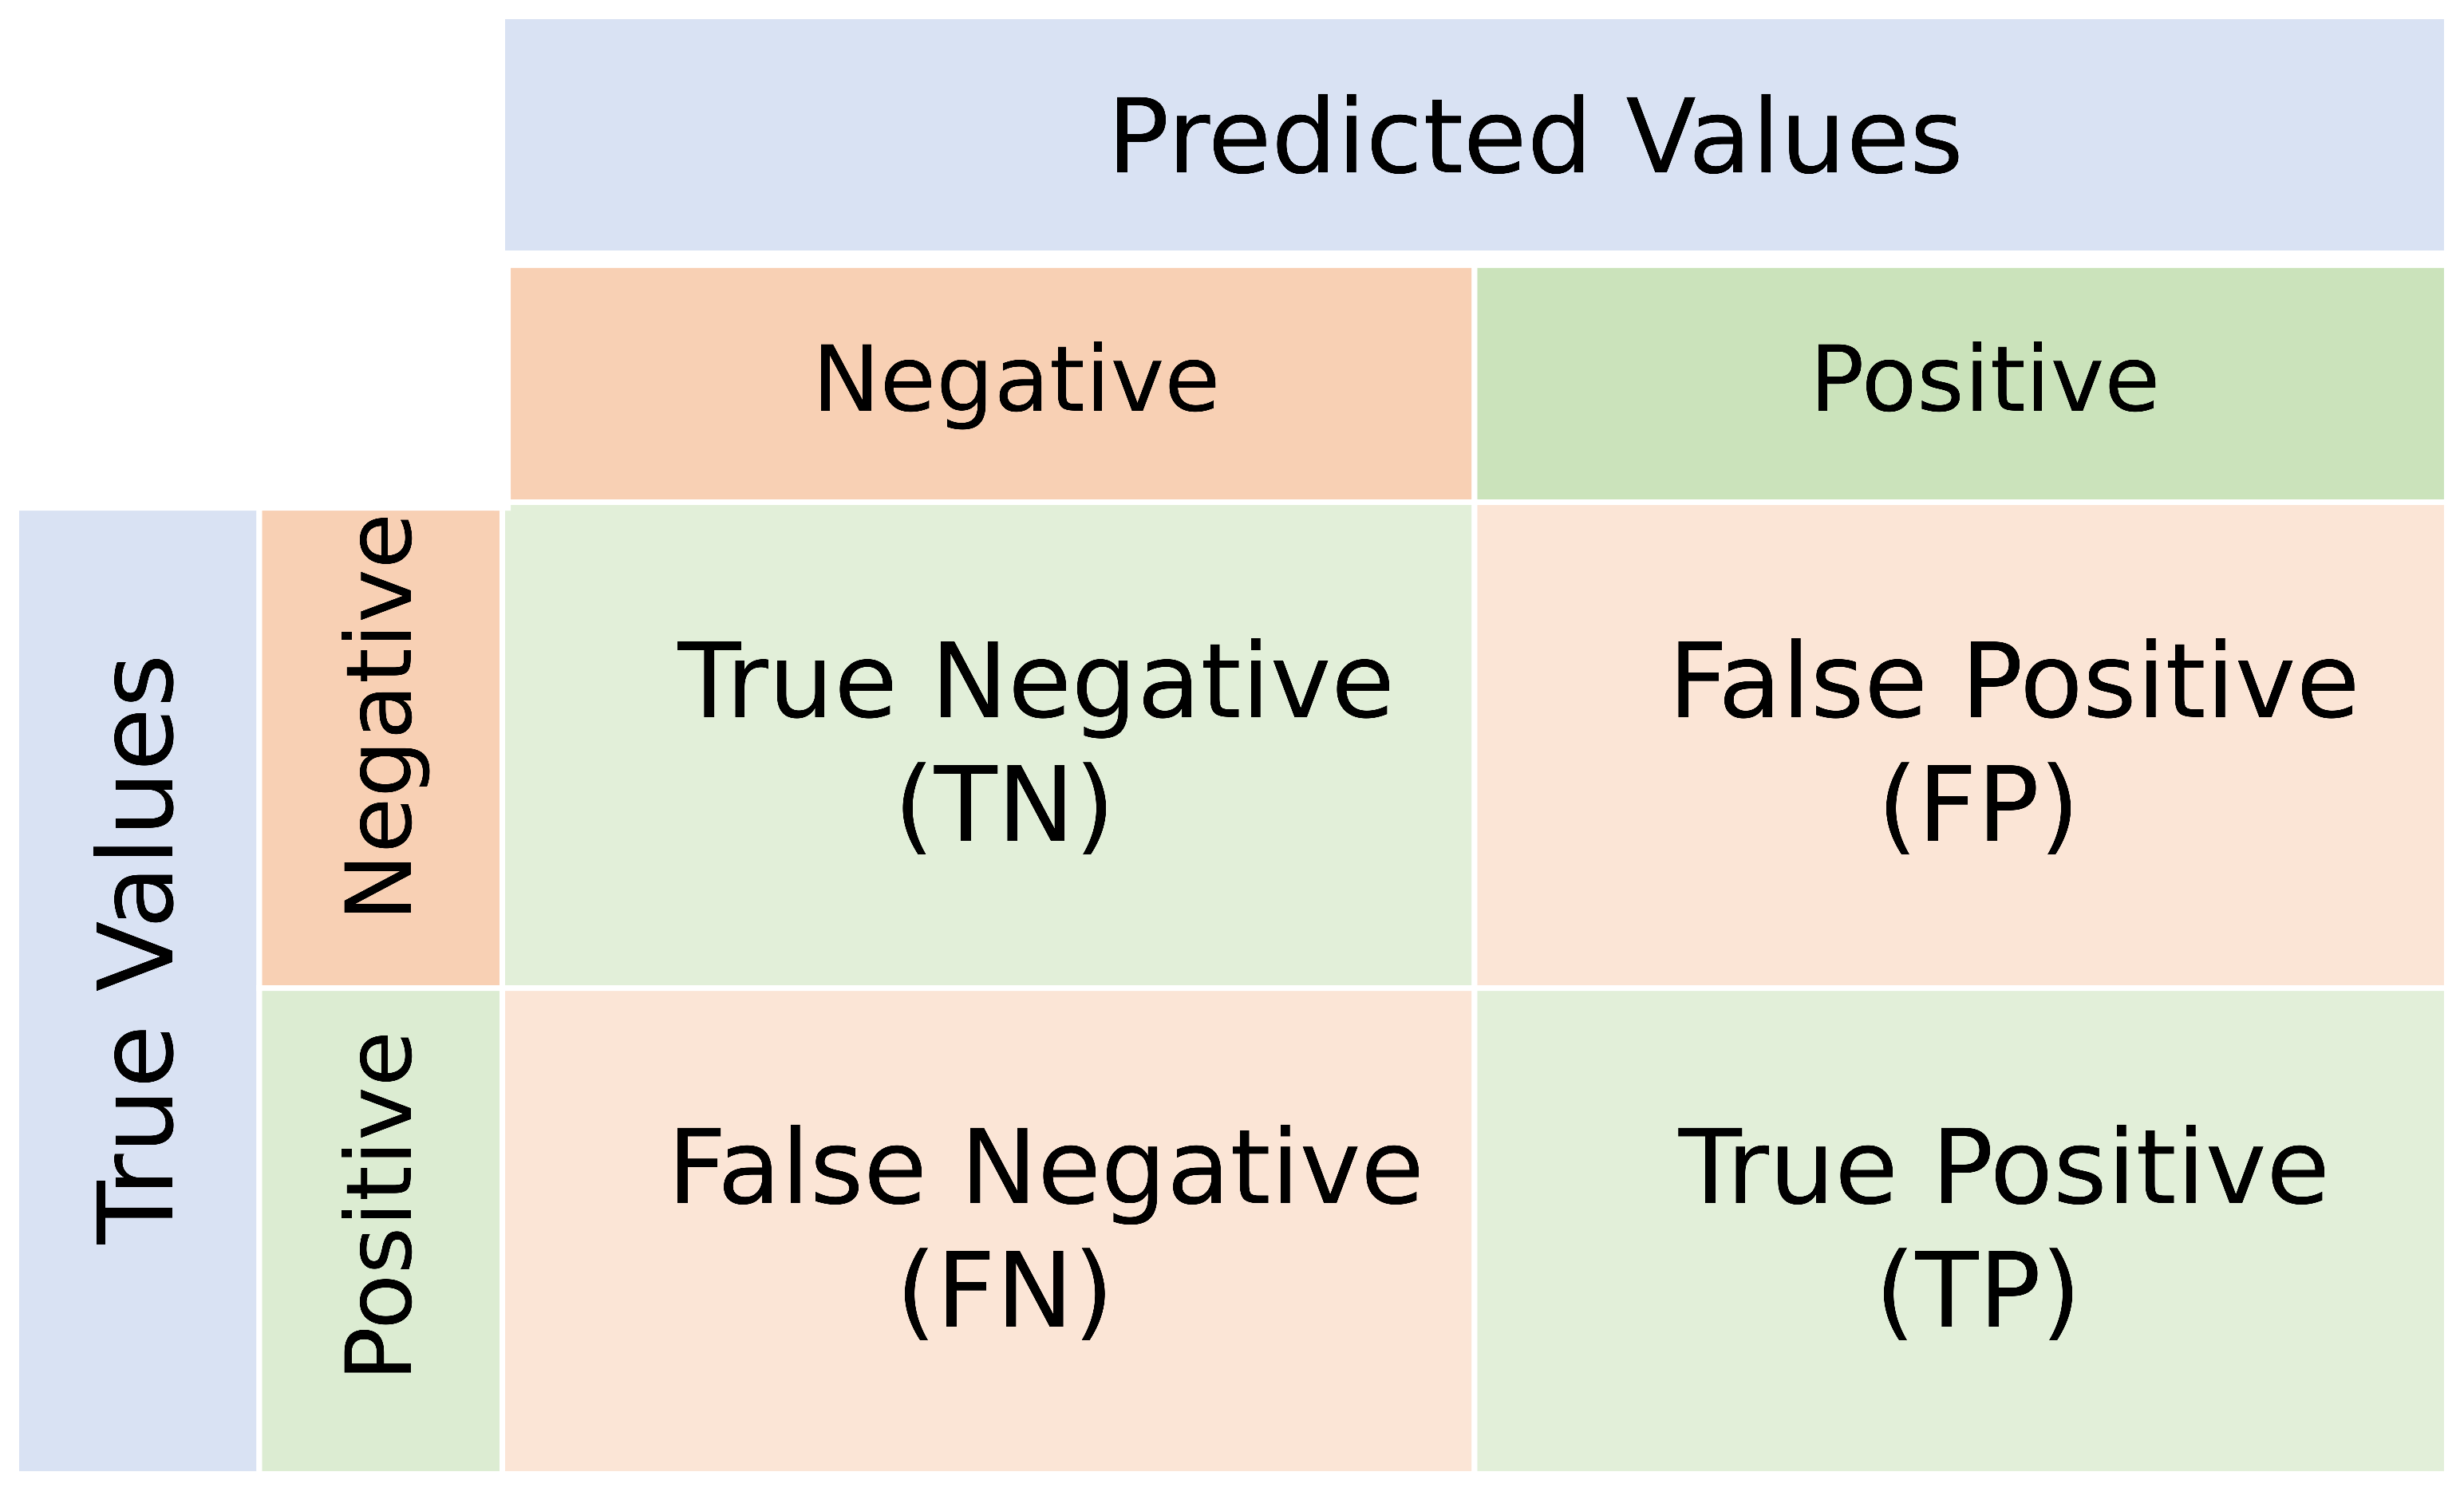
\includegraphics[width=0.5\linewidth]{../img/confusion matrix.eps}
      \caption{Confusion Matrix}
      \label{fig:confusion matrix}
\end{figure}

The confusion matrix is constructed based on the predicted results made by the classifier and the true labels of the samples. It provides a breakdown of the samples into four categories:

\begin{itemize}
      \item True Positive (TP): the number of positive examples classified accurately
      \item False Positive (FP): the number of actual negative examples classified as positive
      \item True Negative (TN): the number of negative examples classified accurately
      \item False Negative (FN): the number of actual positive examples classified as negative
\end{itemize}

Accuracy, precision, recall and F1 score are used as performance metrics to evaluate the model. 

Accuracy is the proportion of samples correctly predicted by the model to the total samples. It is obtained by quoting the number of correct samples in the prediction with the number of overall samples.

\begin{eqnarray}
      Accuracy = \frac{TP + TN}{TP + TN + FP + FN}
      \label{acc}
\end{eqnarray}

Precision measures the proportion of correctly predicted positive samples to the total number of positive predictions made by the model. It assesses the model's ability to avoid false positive predictions.

\begin{eqnarray}
      Precision = \frac{TP}{TP + FP}
      \label{pre}
\end{eqnarray}

Recall is the proportion of the number of positive samples correctly predicted by the model to the number of all positive samples in the dataset. It evaluates the model's ability to identify all positive samples.

\begin{eqnarray}
      Recall = \frac{TP}{TP + FN}
      \label{rec}
\end{eqnarray}

The F1 score is the harmonic mean of the precision and recall. It provides a balanced measure of a model's performance by considering both precision and recall simultaneously.

\begin{eqnarray}
      \begin{aligned}
            Precision &= \frac{2\ast Precision \ast Recall}{Precision + Recall} \\
                      &= \frac{2\ast TP}{2 TP + FP + FN}
      \end{aligned}
      \label{f1s}
\end{eqnarray}


% -----------------------------------------------------------------------------

\chapter{Baseline Model}
\label{chap:execution1}

\noindent
This chapter will cover an approach to sentiment classification based on baseline model. The initial section ooutlines how to pre-process the data, and transform textual data into a format compatible with the model. Subsequently, the second section contains an explanation of the baseline model. Moving forward, the third section tries to enhance the model performance by optimising the data processing part based through the utilization of word embedding. Following this, the fourth section evaluates the model through the analysis of the performance metrics. Finally, the last section includes the explanation of the model, dissecting the factors contributing to both its good and bad performances.

\section{Preprocess Data}
\noindent
Since algorithms can only handle numeric data, data preprocessing is essential to enable text data to be received by the model and facilitate learning features. Raw text often contains a lot of redundant and repetitive information, while data preprocessing can help the algorithm to focus on the core content of the text, which improves the accuracy of the algorithm.

\subsection{Exploratory Data Analysis}
\noindent
Firstly, the entire dataset undergoes the test to see whether it is balanced or not, and if there are any missing values. Alongside the length distribution within each category is analyzed. Upon dataset examination, it's revealed that the label consists of two categories: "suicide" and "non-suicide". The sample size of both categories is 116,037 entries, which is a balanced dataset with no missing values. However, there's significant variance in the average data length between categories. Figure \ref{fig:describe} depicts the relationship between sample length, in terms of the number of tokens, and sample numbers. 

\begin{figure}[h]
      \centering
      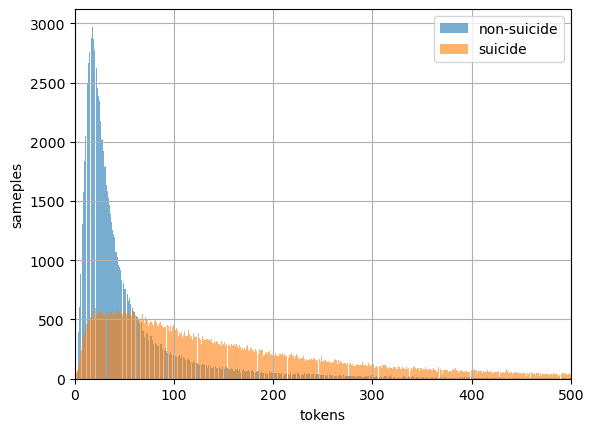
\includegraphics[width=0.6\linewidth]{../img/data_describe.png}
      \caption{Distribution of Data across Samples of Varying Lengths}
      \label{fig:describe}
\end{figure}

Notably, the average sample length in the "suicide" category exceeds that of the "non-suicide" category. The specific data is shown in the Table \ref{tab:describe}.

\begin{table}[h]
      \centering
      \begin{tabular}{ccccc}
            \hline
            class & count & mean length & min & max \\
            \hline
            suicide & 116037 & 61.188 & 2 & 8220 \\
            non-suicide & 116037 & 202.662 & 1 & 9684 \\
            \hline
      \end{tabular}
      \caption{Data Description}
      \label{tab:describe}
\end{table}

Following the initial analysis, word clouds were generated for each of the two categories of data. A word cloud offers a visual depiction of word frequency. The more frequently a word occurs within the text being analysed, the larger that word is in the generated image. This visualization technique is increasingly being used as a simple tool for determining the focus of written material.\cite{atenstaedt2012word} Figure \ref{fig:word cloud} shows the word cloud of both "non-suicide"(Figure \ref{fig:word cloud}\ref{sub@wc_n}) and "suicide"(Figure \ref{fig:word cloud}\ref{sub@wc_s}) categories.

\begin{figure}[h]
      \centering
      \subfloat["non-suicide" Class]{
            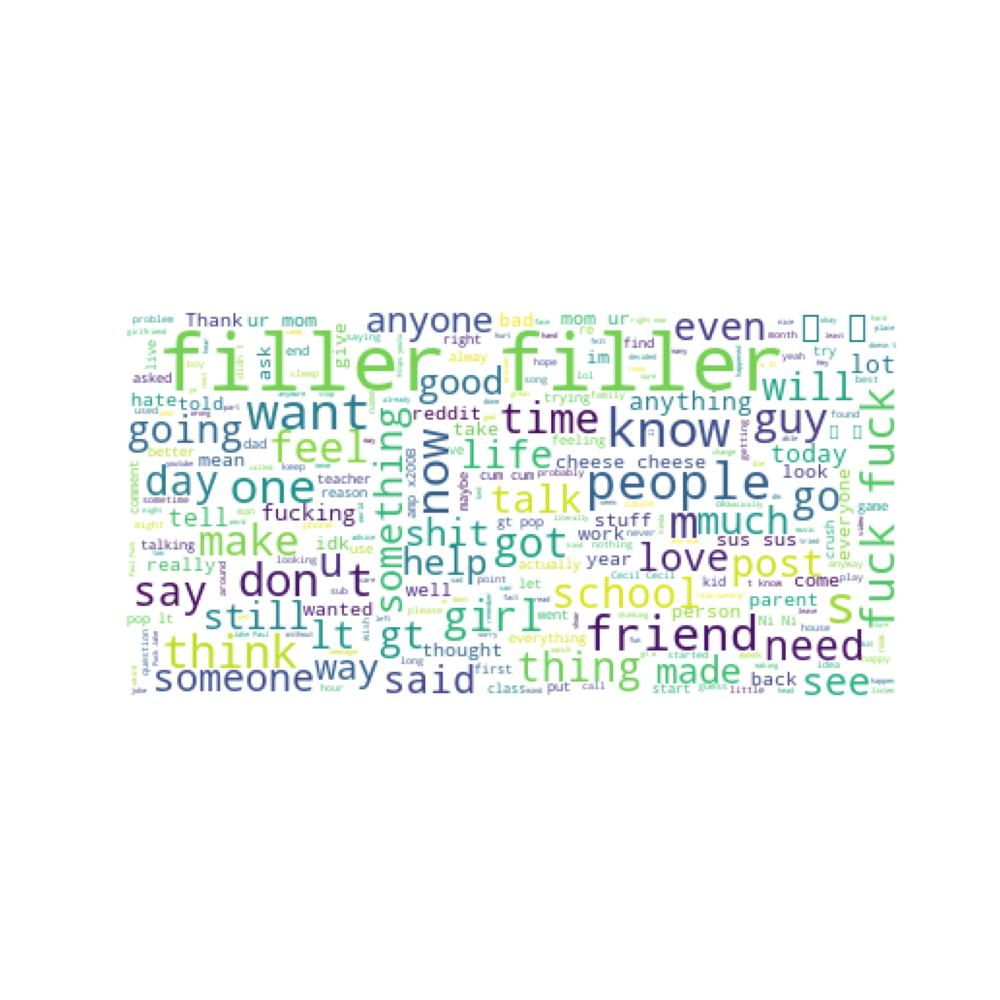
\includegraphics[width=0.44\linewidth]{../img/wc_nonsuicide.jpg}
            \label{wc_n}}
      \hfil
      \subfloat["suicide" Class]{
            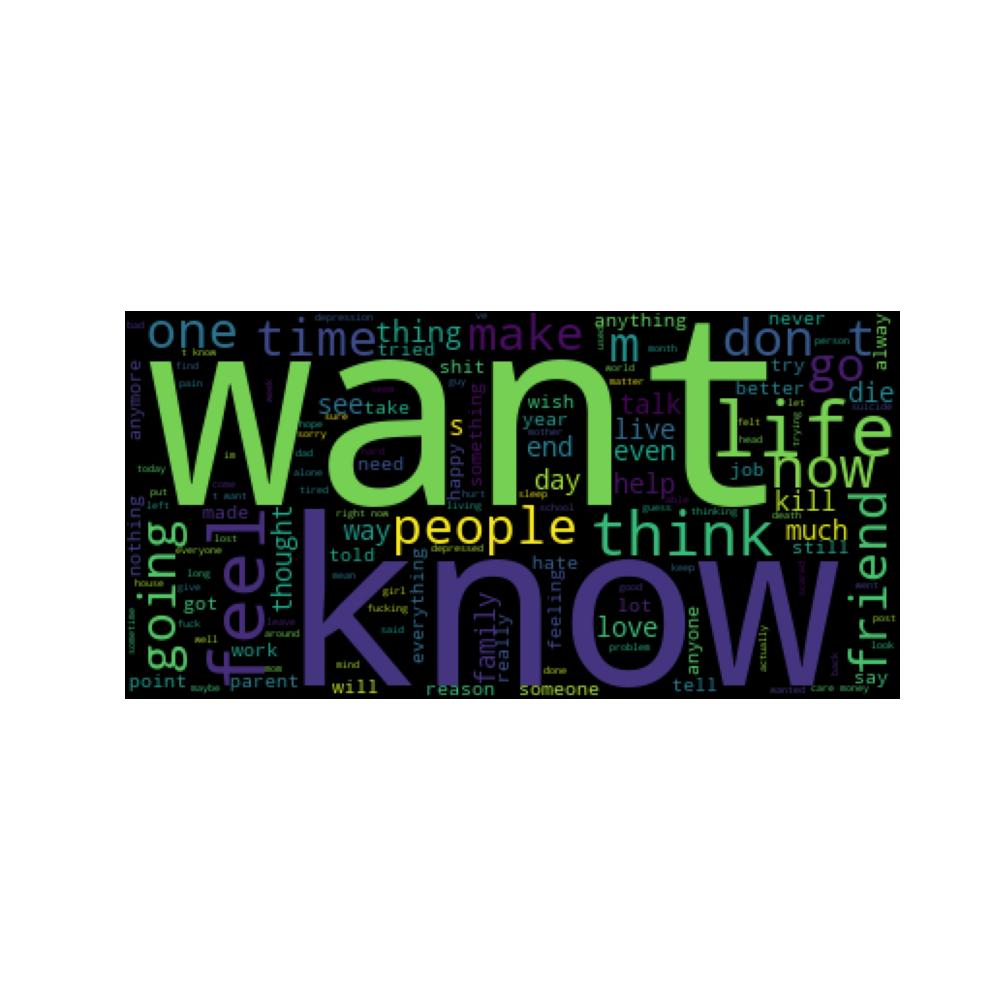
\includegraphics[width=0.44\linewidth]{../img/wc_suicide.jpg}
            \label{wc_s}}
      \caption{Word Cloud of both two Categories of Raw Texts}
      \label{fig:word cloud}
\end{figure}

\subsection{Data Cleaning}
\noindent
After performing exploratory data analysis, a general understanding of the data set has been obtained. The next step should be to preprocess the data.

Missing values can appear due to various reasons, such as data entry errors, sensor failures, or simply due to the nature of the data collection process. Common processing methods to deal with missing values include deletion, filling with special values, marking as a new class, and so on. The section of a method depends on the characteristics of the dataset and the most appropriate method must be chosen accordingly. However, since there are no missing values in this dataset, this step is not required.

Given the presence of numerous abbreviations in the text, which may lead to interpretational confusion. Therefore it is essential to convert common abbreviations into their full forms. This can be handled with a dictionary structure in Python, containing common abbreviations and corresponding full forms. Each word in the text can then be iterated through regular expressions and the abbreviations contained in the dictionary are replaced.

What's more, the dataset may contain many unwanted content such as URLs, emojis, special symbols, etc. These are not conductive to semantic analysis of the text and may even interfere with the learning process of the model. Such content can be filtered out with regular expressions.

Finally, it is vital to remove the stopwords in the text. Stopwords are words that appear frequently in the text (e.g., "the", "is", "and") but contribute minimally to the meaning of the text. Removing these words can enhance text processing efficiency. Many organisations published their pre-made stopwords lists. Here the English stopword list provided by the NLTK library is used to remove stopwords from the dataset.

Subsequently, Figure \ref{fig:word cloud clean} shows the word cloud of the dataset extracted after data cleaning to compare the result before and after data cleaning.

\begin{figure}[h]
      \centering
      \subfloat["non-suicide" Class after Cleaning]{
            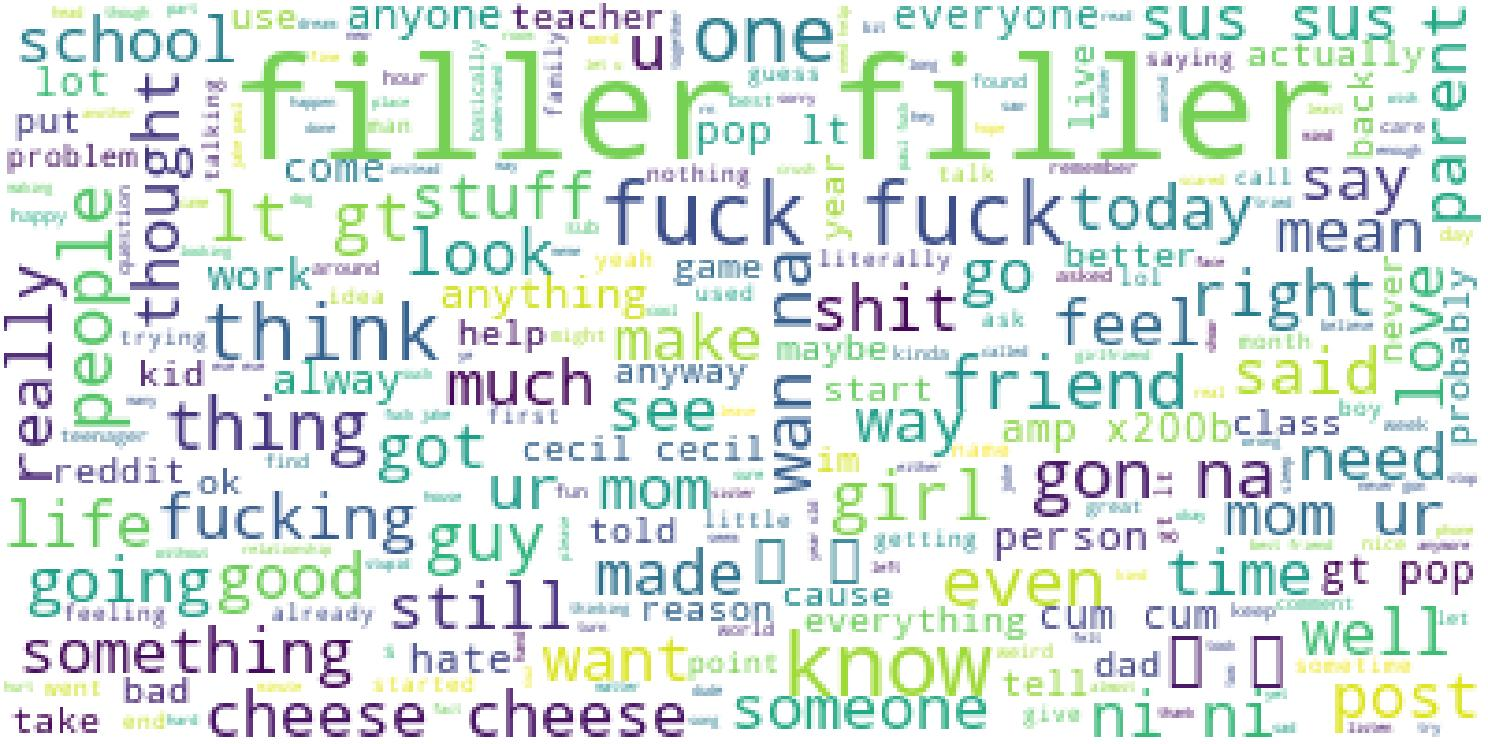
\includegraphics[width=0.44\linewidth]{../img/wc_nonsuicide_c.jpg}
            \label{wc_n_c}}
      \hfil
      \subfloat["suicide" Class after Cleaning]{
            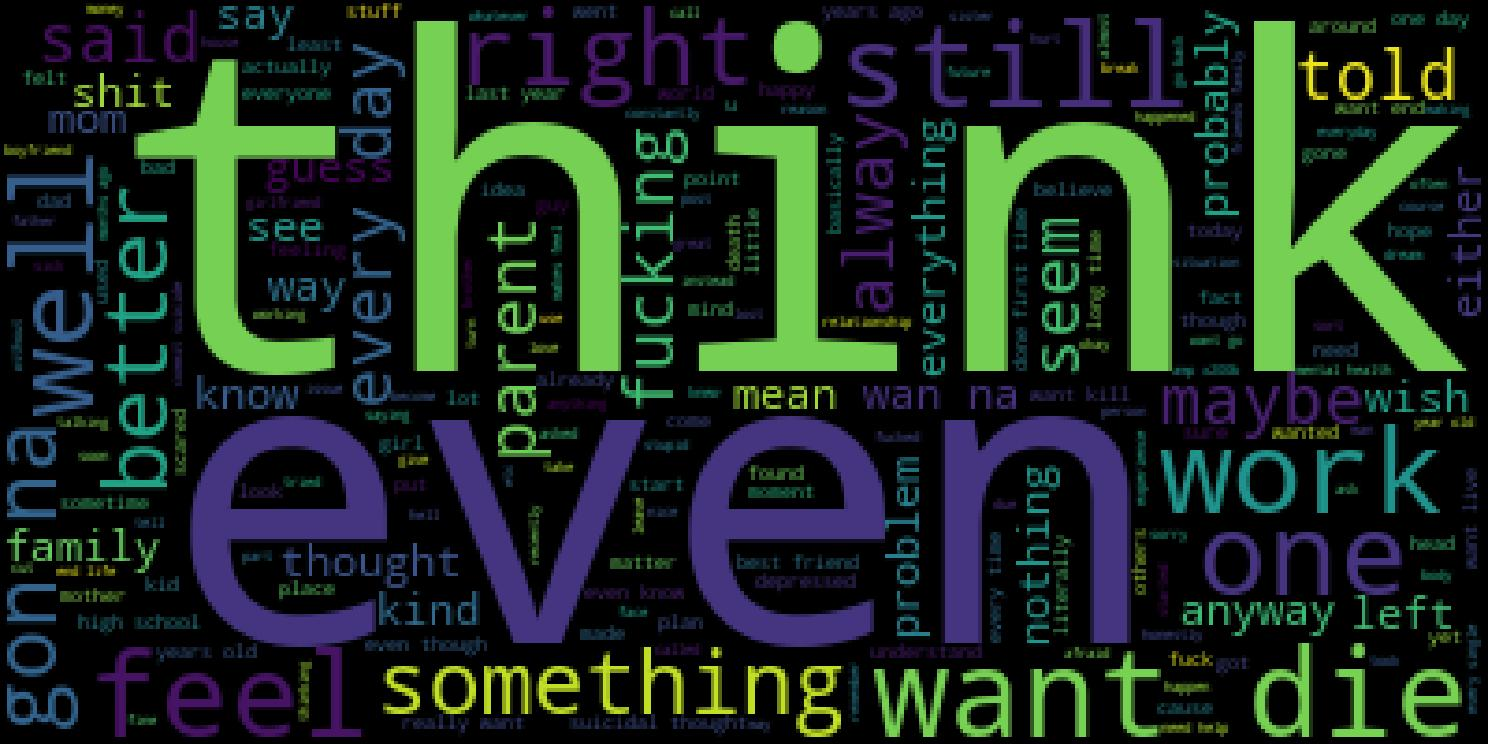
\includegraphics[width=0.44\linewidth]{../img/wc_suicide_c.jpg}
            \label{wc_s_c}}
      \caption{Word Cloud of both two Categories after Data Cleaning}
      \label{fig:word cloud clean}
\end{figure}

\subsection{Word Vectorization}
\noindent
After cleaning the dataset, the text needs to be vectorially represented. BoW model is one of the commonly used vector representation models among so many models. BoW model, based on one-hot encoding\cite{chren1998one}, is a simple yet powerful technique used in NLP for representing text data. It's based on the concept of treating text as a "bag" of individual words, disregarding grammar and word order, and focusing solely on word frequency. The workflow of the model is divided into the following steps:

\begin{enumerate}
      \item Tokenization: The first step is to break down the text into individual tokens. This process involves splitting the text into words based on whitespace characters.
      \item Vocabulary Creation: Next, a vocabulary is created by compiling a list of unique words present in the entire dataset. Each unique word in the vocabulary becomes a feature in the BoW model.
      \item Vectorization: For each document in the dataset, a vector is constructed where each element represents the frequency of a word from the vocabulary in that document. The length of the vector is equal to the size of the vocabulary, and the values are the counts of each words in a document.
      \item Sparse Representation: Since most documents only contain a small subset of the words in the vocabulary, the resulting vectors are typically sparse, meaning that most of the elements are zero.
\end{enumerate}

During implementation, the maximum number of features can be set to prevent excessive dimensionality and to speed up processing. Finally a sparse matrix representing the number of occurrences of the word will be obtained as the word vector passed to the model.

\section{Logistic Regression}
\noindent
After the data pre-processing step, a vector-like representation of the data is obtained, which can be served as the training and testing data for the baseline model. Here, logistic regression is used as the baseline model. Logistic regression is a classification method in the field of statistics and machine learning. Despite its name, logistic regression is a classification algorithm, not a regression algorithm. The goal of logistic regression is to predict the probability of an event occurring, achieved through a combination of linear regression and an activation function.

As a generalized linear regression algorithm, logistic regression initially employs a linear regression algorithm to model the relationship between the independent (features) and dependent (outcome) variables. The linear equation takes the following form:

\begin{eqnarray}
      z=b_0+b_1x_1+b_2x_2+\cdots+b_nx_n
      \label{Linear Regression}
\end{eqnarray}

Where $z$ represents the log-odds of the probability of the positive class, $x_1,x_2,\cdots,x_n$ are the feature variables, and $b_1,b_2,\cdots,b_n$ are the coefficients to be estimated. The linear result $z$ is next passed to a logistic function that converts the log odds into a probability ranging between 0 and 1. The sigmoid function is most commonly used for this transformation, defined as:

\begin{eqnarray}
      p(z)=\frac{1}{1 + e^{-z}}
      \label{Sigmoid Function}
\end{eqnarray}

Where $p$ represents the probability of a positive prediction. The complete logistic regression formula can be obtained by combining the two formulas:
\begin{eqnarray}
      p=\frac{1}{1 + e^{-(b_0+b_1x_1+b_2x_2+\cdots+b_nx_n)}}
      \label{Logistic Regression}
\end{eqnarray}

After that, a threshold is determined to serve as a dividing line (usually 0.5), making the predicted probability converted into a binary outcome. If the predicted probability is greater than the threshold, the instance is classified as belonging to the positive class; otherwise, it is classified as belonging to the negative class.

Logistic regression iteratively updates the coefficients $b_1,b_2,\cdots,b_n$ through optimisation algorithms such as maximum likelihood estimation (MSE) or stochastic gradient descent (SGD). The objective is to adjust the coefficients in such a way that the probability of positive category increased and the probability of negative category decreased. This iterative optimization process continues until convergence, where the model parameters converge to their optimal values, leading to the best model performance.

\section{Improve with Word Embedding}
\noindent
Considering the large size of the dataset, the dimensionality of the BoW model escalates, resulting in what is commonly referred to as a "dimensional disaster". And it lacks the ability to capture relationships between words, which is poor for semantic extraction. Compared to the BoW model, the word embedding approach offers a solution by mapping words to a fixed-dimensional vector space, which is much smaller than the vocabulary's dimension. This facilitates the evaluation of semantic proximity among various words in the vector space, while also encompassing contextual nuances to differentiate between disparate meanings of the same word across contexts. Consequently, word embedding is applied to try to improve the model performance.

As one of the current mainstream pre-training models, BERT is pre-trained with a large number of samples and has good performances in many tasks. Therefore the tokenizer and word embedding methods provided by BERT are used to process the text data.

\subsection{Tokenize}
\noindent
In order to help the model understand the text and discern each word within a sentence, a tokenizer is employed to break the text into small tokens, which are subsequently transformed into word vectors. While the previously mentioned BoW model typically separates tokens based on spaces, it encounters challenges with words exhibiting various forms, such as tense or plurality. Moreover, space is not used to segment words in many language like Chinese, so this method is not universally applicable. In order to improve the word tokenization method, the subword-based method is introduced. This method combines small subwords to form larger words, mitigating the need to tokenize every word individually from an extensive dataset. For example, "transformer" can be segmented into "transform" + "er", which is more flexible and adaptive. BERT uses the WordPiece algorithm\cite{wu2016google}, one of the subword-based methods, for its tokenizer, segmenting the word "transformer" into "transform" + "\#\#er". The "\#\#" of the latter token indicates that it is part of the former word.

To helping effectively utilizing BERT model in different NLP tasks, Bert Tokenizer adds some special tokens to the text:

\begin{itemize}
      \item\ [CLS]: Added at the beginning of a sequence, usually for classification tasks.
      \item\ [SEP]: Added at the end of a sequence to separate sentences or mark the end of a sentence pair.
      \item\ [PAD]: Used to fill the sequence to a uniform length.
      \item\ [UNK]: Used to represent words outside the BERT vocabulary, enhancing the model's ability to generalise to new words.
      \item\ [MASK]: Used in pre-training for masking language modelling tasks.
\end{itemize}

After the split, the tokeniser converts the text into a format that the BERT model can understand. This method returns a dictionary containing the following:

\begin{itemize}
      \item input\_ids: a sequence of ids for the token string, based on the vocabulary
      \item attention\_mask: indicates which tokens are valid and which are padded
      \item token\_type\_ids: sequences that distinguish different sentences in a sentence pair (if it is a sentence pair)
\end{itemize}

\subsection{Word Embedding}
\noindent
Like many other deep learning models in NLP, BERT processes the words in the text through the token embedding layer to convert them into word vectors. However, unlike conventional models, BERT has two additional embedding layers, the segment embedding layer and the position embedding layer. This unique architecture of the BERT embedding layer is depicted in the Figure \ref{fig:bert_embedding}.

\begin{figure}[h]
      \centering
      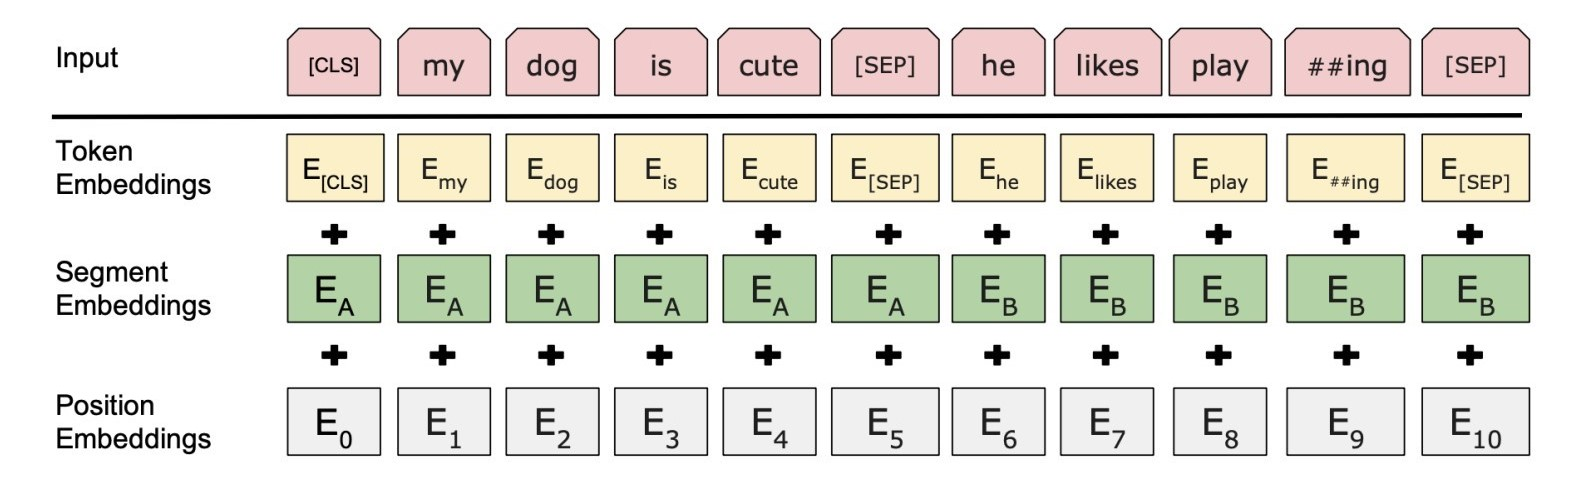
\includegraphics[width=0.6\linewidth]{../img/bert_embedding.jpg}
      \caption[BERT Input Representation]{BERT Input Representation.\cite{devlin2018bert}}
      \label{fig:bert_embedding}
\end{figure}

Token Embeddings: Encode the word IDs and convert them into fixed-dimensional vectors. In BERT, each word is typically transformed into a 768-dimensional vector representation by default. Suppose $batch\_size$ represents the size of a batch and $sen\_length$ represents the number of tokens in a sentence, the input dimension is $[batch\_size, sen\_length]$ and dimension of the output tensor is $[batch\_size, sen\_length, 768]$.

Segment Embeddings: Useful only when the input is a sentence pair, it helps BERT to distinguish whether a token belongs to the first sentence or the second sentence. When only one sentence is input, the segment embedding values of each token are $0$. When two sentences are input, tokens from the first sentence are assigned a segment embedding value of $0$, while tokens from the second sentence are assigned a value of $1$.

Position Embeddings: Facilitate BERT in learning the sequential order of input tokens. Because of Transformers' inability to handle sequence positions, position information need to be added manually to ensure proper sequence handling.

The three embedding results are summed without weights with a size of $[batch\_size, sen\_length, 768]$. BERT applies layer normalisation to adjust the resultant tensor\cite{pymars2020normalisation}, which contributes to the stability and efficiency of model training. Finally, BERT applies dropout technique to regularise the model and reduce the risk of overfitting.

\section{Baseline Performance}
\noindent
The dataset is split into a training set and a test set in the ratio of 8:2. The training set is utilized to train the model so that it can learn the relationships within the data, enabling the model to perform well on the target task. The test set is not involved in the training process and is reserved as unseen data. This separation simulates real-world scenarios where the model encounters new, unseen data for prediction. By evaluating the model's performance on the test set, its predictive capability under real-world conditions can be assessed.

To ensure the accuracy and reliability of the results, a stratified K-fold cross-validation approach is employed on the training set\cite{browne2000cross}. The entire training set is divided into $K$ equal-sized subsets, known as "folds". Moreover, each fold maintains the same proportion of samples in each category as in the original dataset, enhancing the robustness of performance estimates. During each iteration of the cross-validation process, one fold is selected as the validation set and the remaining serve as the training set to evaluate the model performance. This process is repeated $K$ times. Finally, the average performance metric of all $K$ iterations is calculated to get the generalisation ability of the model. In this experiment the value of $K$ is chosen as $5$. The structure of the cross validation process is showen in Figure \ref{fig:cross validation}.

\begin{figure}[h]
      \centering
      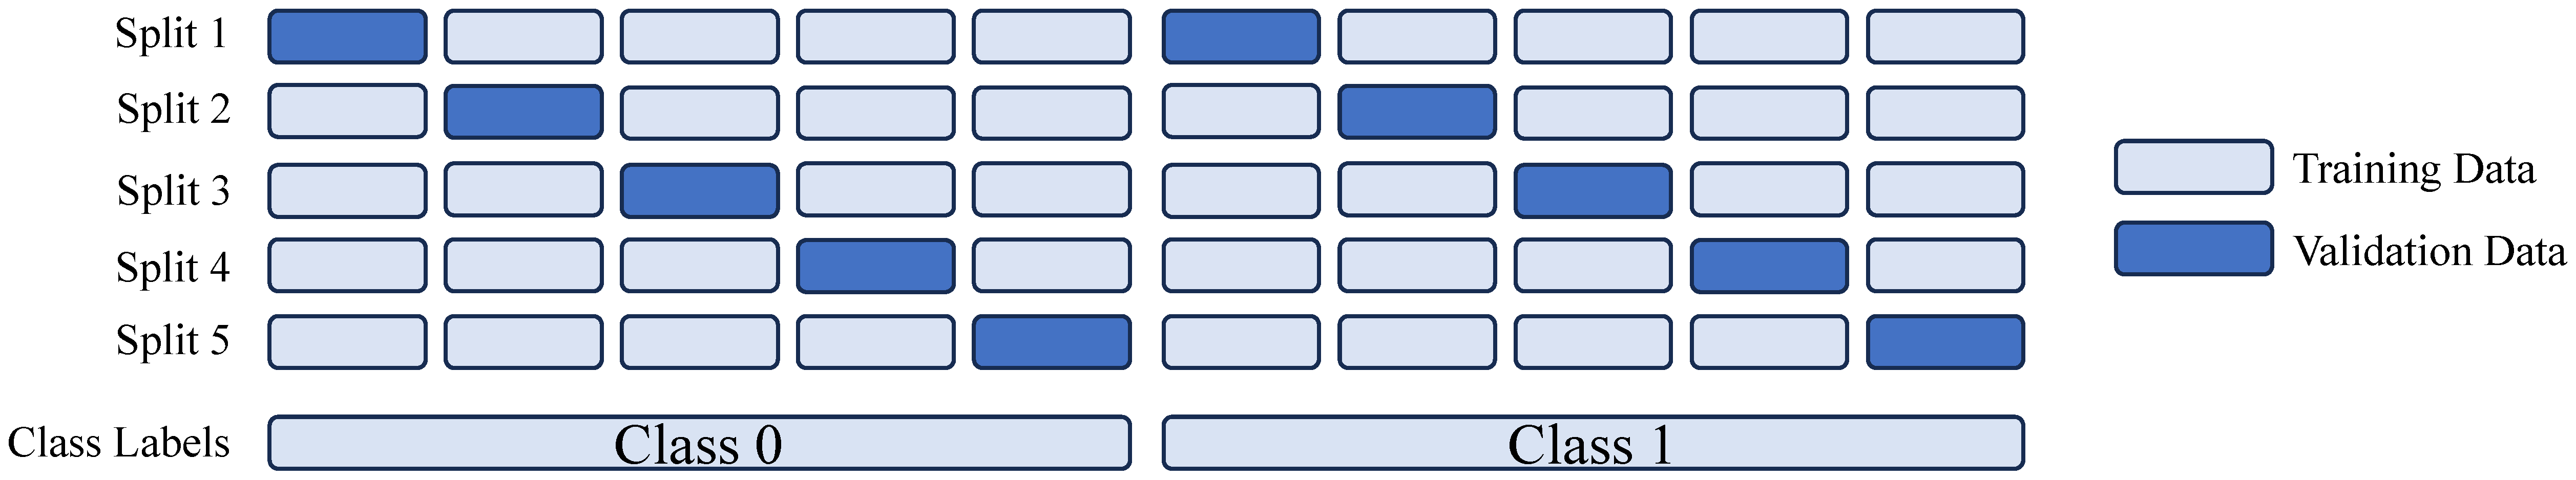
\includegraphics[width=0.7\linewidth]{../img/cv.eps}
      \caption{Stratified K-Fold Cross Validation}
      \label{fig:cross validation}
\end{figure}

\subsection{Logistic Regression with CountVectorizer}

\subsection{Logistic Regression with BERT Embedding}

\section{Baseline Model Explanation}

% -----------------------------------------------------------------------------

\chapter{Deep Learning Model}
\label{chap:execution2}
\noindent

\section{Recurrent Neural Network}

\subsection{Bi-LSTM Model}

\subsection{Bi-LSTM Model Performance}

\subsection{Bi-LSTM Model Explanation}

\section{Large Language Model}

\subsection{BERTForSequenceClassification}

\subsection{BERT Model Performance}

\subsection{BERT Model Explanation}

% -----------------------------------------------------------------------------

\chapter{Suicide Ideation Identification System Implementation}
\label{chap:implementation}

% -----------------------------------------------------------------------------

\chapter{Conclusion}
\label{chap:conclusion}

\section{Summary}

\noindent

\section{Project Status}

\noindent
The aims of the project are as follows:

\begin{itemize}
      \item one
      \item two
\end{itemize}

\section{Further Work}

\noindent

\textbf{one}

\textbf{two}


% =============================================================================

% Finally, after the main matter, the back matter is specified.  This is
% typically populated with just the bibliography.  LaTeX deals with these
% in one of two ways, namely
%
% - inline, which roughly means the author specifies entries using the 
%   \bibitem macro and typesets them manually, or
% - using BiBTeX, which means entries are contained in a separate file
%   (which is essentially a database) then imported; this is the 
%   approach used below, with the databased being dissertation.bib.
%
% Either way, the each entry has a key (or identifier) which can be used
% in the main matter to cite it, e.g., \cite{X}, \cite[Chapter 2}{Y}.

\backmatter

\bibliography{sample_bibtex.bib}

% -----------------------------------------------------------------------------

% The dissertation concludes with a set of (optional) appendices; these are 
% the same as chapters in a sense, but once signalled as being appendices via
% the associated macro, LaTeX manages them appropriately.

\appendix

\chapter{Appendix}
\label{appx:example}

Content which is not central to, but may enhance the dissertation can be 
included in one or more appendices; examples include, but are not limited
to

\begin{itemize}
\item lengthy mathematical proofs, numerical or graphical results which 
      are summarised in the main body,
\item sample or example calculations, 
      and
\item results of user studies or questionnaires.
\end{itemize}

\noindent
Note that in line with most research conferences, the examiners are not
obliged to read such appendices.

% =============================================================================

\end{document}
